% huscs, N=32*32*32, numThreadsPerLocale=1, step=1
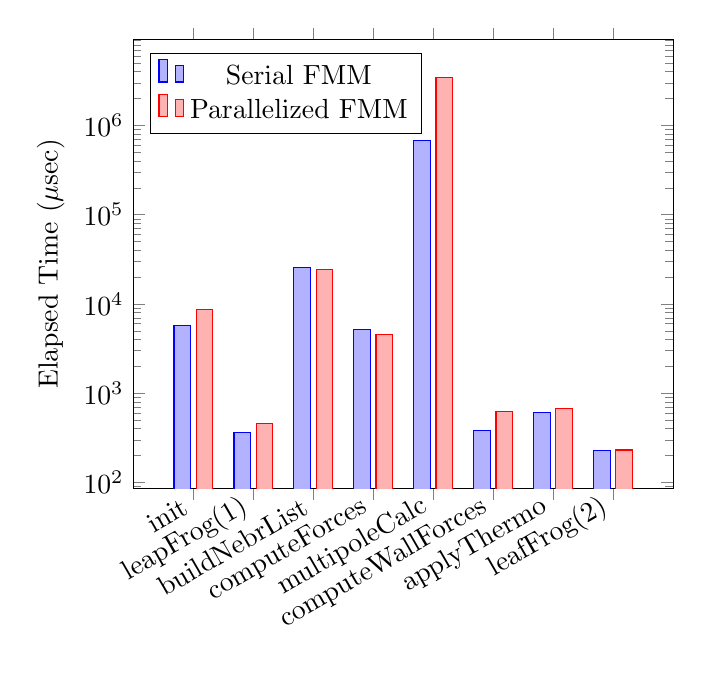
\begin{tikzpicture}
\begin{axis}[
  ymode=log, ybar, bar width=6pt,
  ylabel=Elapsed Time ($\mu$sec),
  xmin=0, xmax=9, xtick={1, 2, 3, 4, 5, 6, 7, 8},
  xticklabels={init, leapFrog(1), buildNebrList, computeForces, multipoleCalc,
    computeWallForces, applyThermo, leafFrog(2)},
  x tick label style={rotate=30, anchor=east},
  legend pos=north west, legend columns=1]
\addplot coordinates
  {(1, 5691) (2, 360) (3, 25388) (4, 5145) (5, 674491) (6, 385) (7, 603) 
   (8, 227)};
\addplot coordinates
  {(1, 8631) (2, 462) (3, 24151) (4, 4550) (5, 3480940) (6, 618) (7, 680) 
   (8, 231)};
\legend{Serial FMM, Parallelized FMM}
\end{axis}
\end{tikzpicture}
